\documentclass[11pt,a4paper]{report}
\usepackage[textwidth=37em,vmargin=30mm]{geometry}
\usepackage{calc,xunicode,amsmath,amssymb,paralist,enumitem,tabu,booktabs,datetime2,xeCJK,xeCJKfntef,listings}
\usepackage{tocloft,fancyhdr,tcolorbox,xcolor,graphicx,eso-pic,xltxtra,xelatexemoji}

\newcommand{\envyear}[0]{2025}
\newcommand{\envdatestr}[0]{2025-09-14}
\newcommand{\envfinaldir}[0]{webdb/2025/20250914/final}

\usepackage[hidelinks]{hyperref}
\hypersetup{
    colorlinks=false,
    pdfpagemode=FullScreen,
    pdftitle={Web Digest - \envdatestr}
}

\setlength{\cftbeforechapskip}{10pt}
\renewcommand{\cftchapfont}{\rmfamily\bfseries\large\raggedright}
\setlength{\cftbeforesecskip}{2pt}
\renewcommand{\cftsecfont}{\sffamily\small\raggedright}

\setdefaultleftmargin{2em}{2em}{1em}{1em}{1em}{1em}

\usepackage{xeCJK,xeCJKfntef}
\xeCJKsetup{PunctStyle=plain,RubberPunctSkip=false,CJKglue=\strut\hskip 0pt plus 0.1em minus 0.05em,CJKecglue=\strut\hskip 0.22em plus 0.2em}
\XeTeXlinebreaklocale "zh"
\XeTeXlinebreakskip = 0pt


\setmainfont{Brygada 1918}
\setromanfont{Brygada 1918}
\setsansfont{IBM Plex Sans}
\setmonofont{JetBrains Mono NL}
\setCJKmainfont{Noto Serif CJK SC}
\setCJKromanfont{Noto Serif CJK SC}
\setCJKsansfont{Noto Sans CJK SC}
\setCJKmonofont{Noto Sans CJK SC}

\setlength{\parindent}{0pt}
\setlength{\parskip}{8pt}
\linespread{1.15}

\lstset{
	basicstyle=\ttfamily\footnotesize,
	numbersep=5pt,
	backgroundcolor=\color{black!5},
	showspaces=false,
	showstringspaces=false,
	showtabs=false,
	tabsize=2,
	captionpos=b,
	breaklines=true,
	breakatwhitespace=true,
	breakautoindent=true,
	linewidth=\textwidth
}






\newcommand{\coverpic}[2]{
    % argv: itemurl, authorname
    Cover photo by #2~~(\href{#1}{#1})
}
\newcommand{\makeheader}[0]{
    \begin{titlepage}
        % \newgeometry{hmargin=15mm,tmargin=21mm,bmargin=12mm}
        \begin{center}
            
            \rmfamily\scshape
            \fontspec{BaskervilleF}
            \fontspec{Old Standard}
            \fontsize{59pt}{70pt}\selectfont
            WEB\hfill DIGEST
            
            \vfill
            % \vskip 30pt
            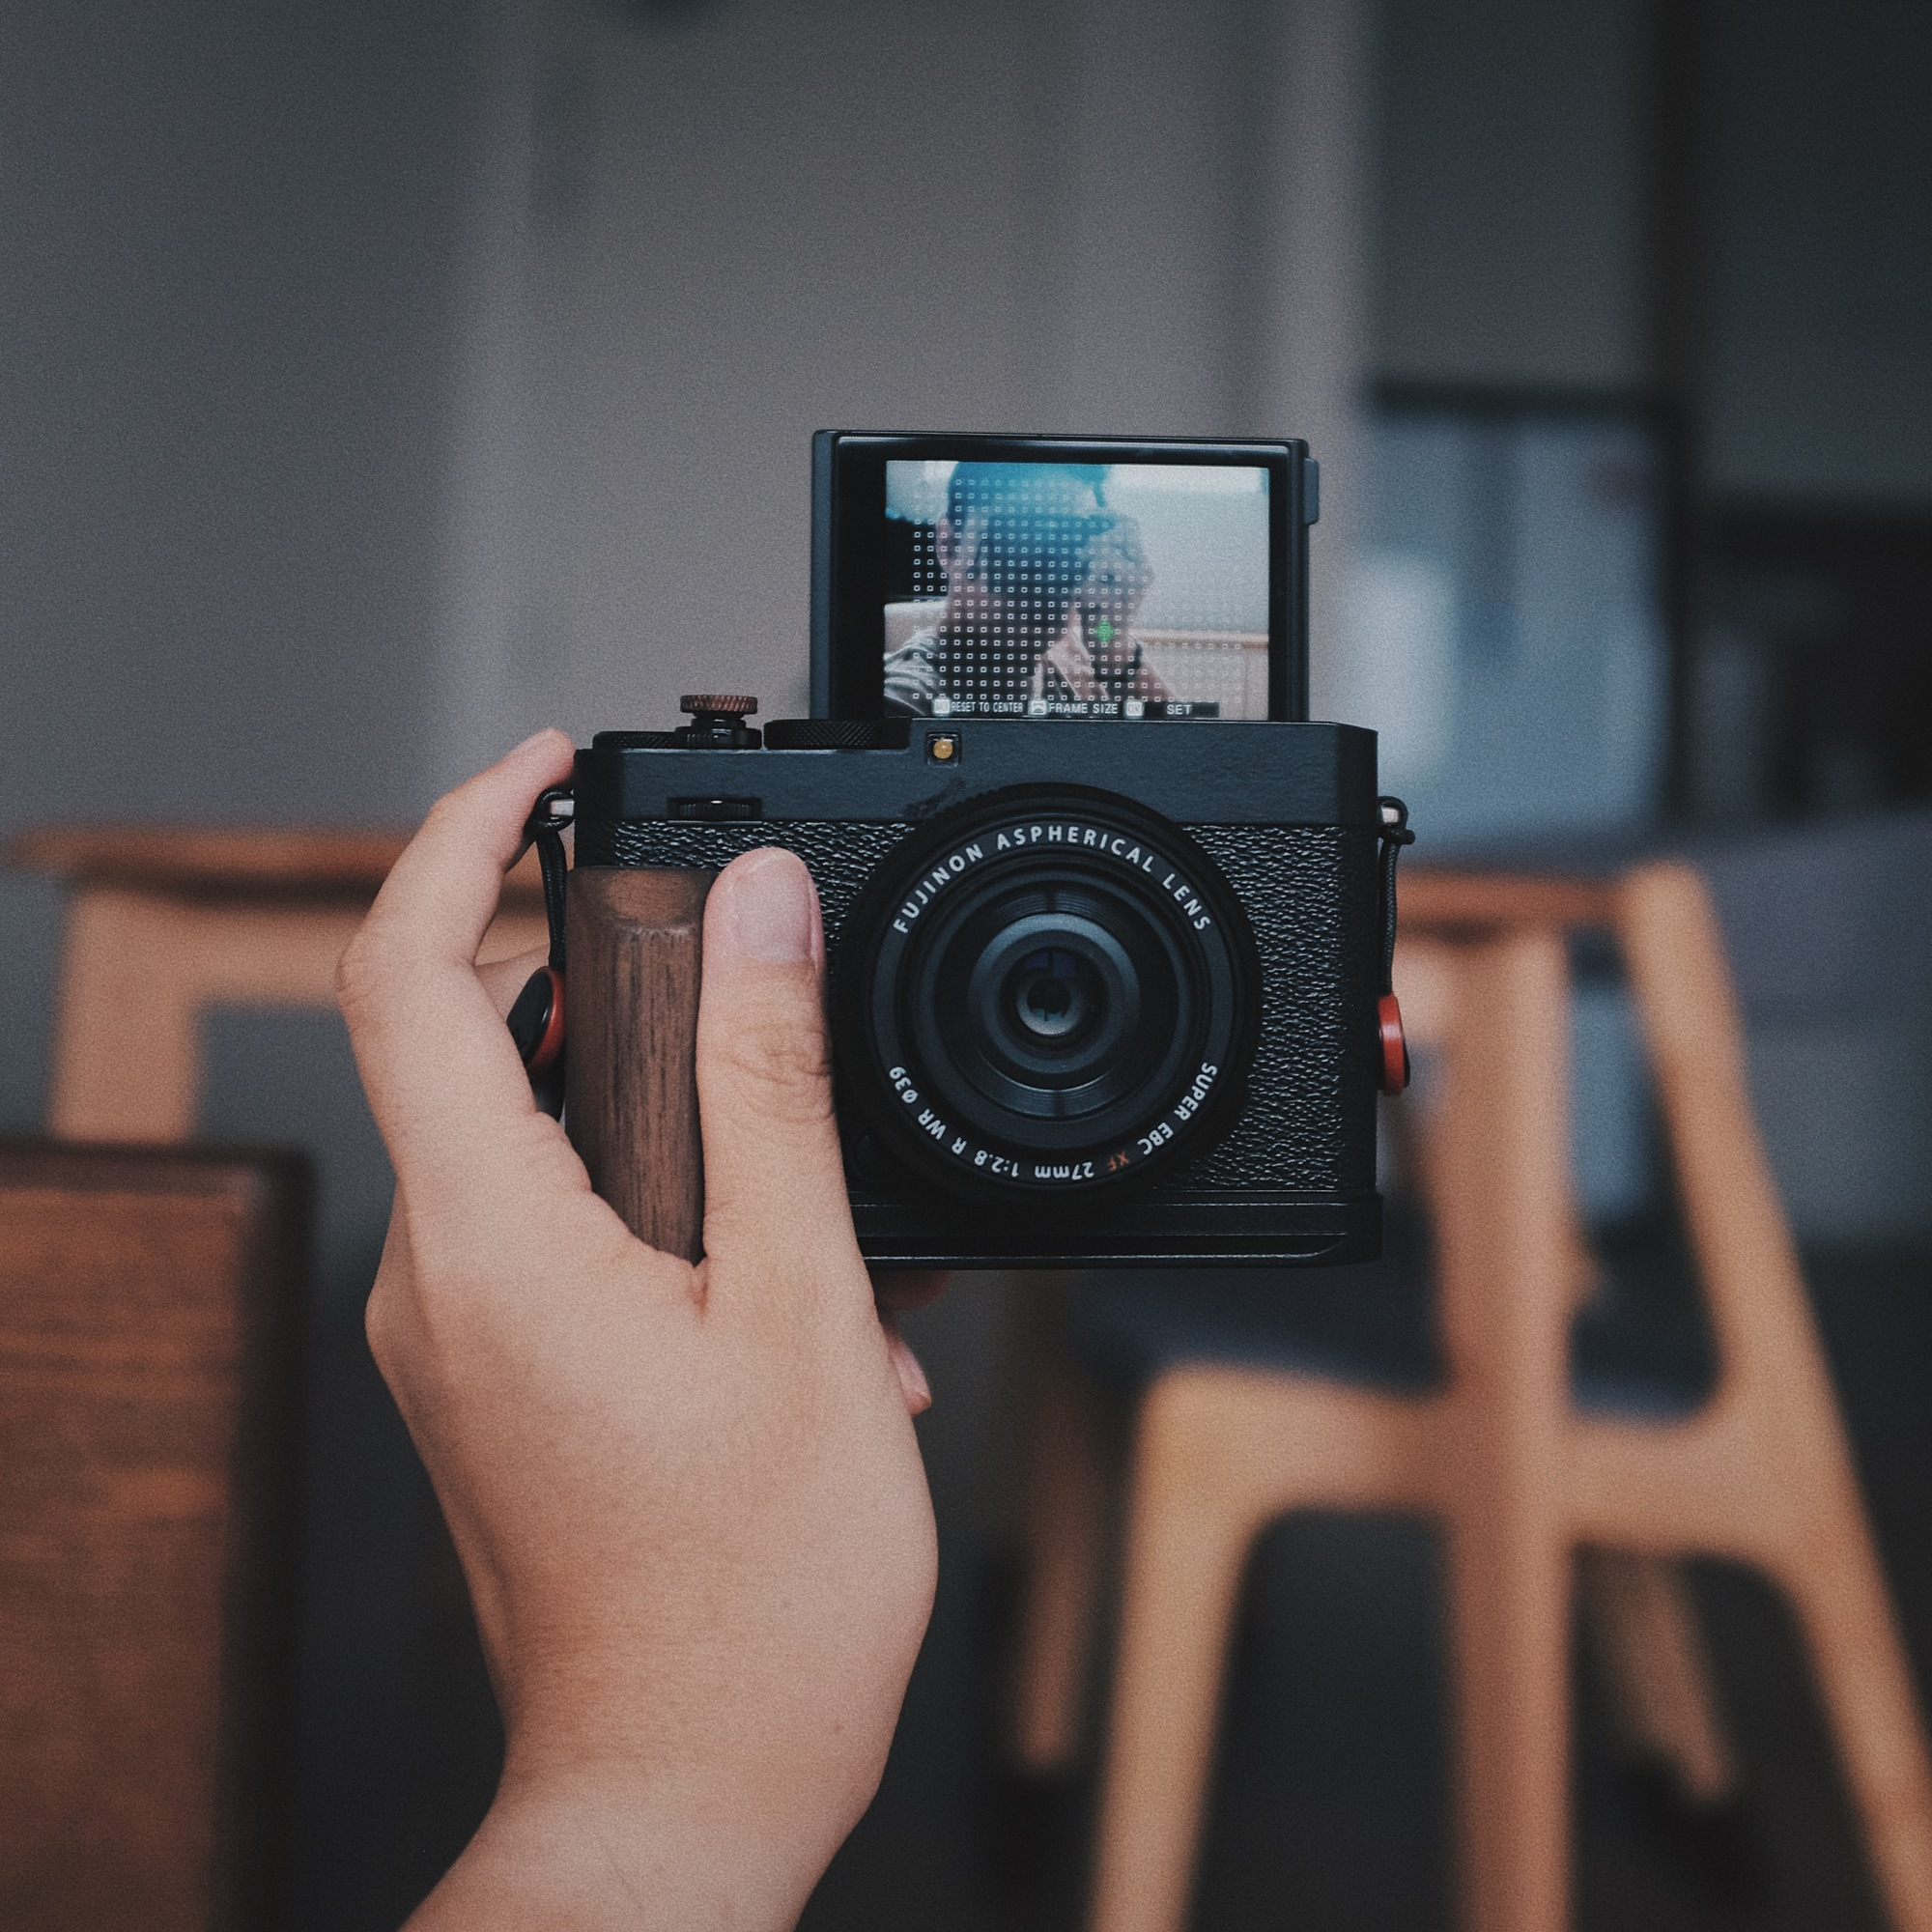
\includegraphics[width=\linewidth]{\envfinaldir/coverpic-prod.jpg}\par
            % \vskip 30pt
            \vfill

            \normalsize\rmfamily\scshape
            \copyright{} The Web Digest Project \hfill\large \envdatestr
        \end{center}
    \end{titlepage}
    % \restoregeometry
}
\newcommand{\simplehref}[1]{%
    \textcolor{blue!80!green}{\href{#1}{#1}}%
}
\renewcommand{\contentsname}{\center\Huge\sffamily\bfseries Contents\par\vskip 20pt}
\newcounter{ipartcounter}
\setcounter{ipartcounter}{0}
\newcommand{\ipart}[1]{
    % \vskip 20pt
    \clearpage
    \stepcounter{ipartcounter}
    \phantomsection
    \addcontentsline{toc}{chapter}{#1}
    % \begin{center}
    %     \Huge
    %     \sffamily\bfseries
    %     #1
    % \end{center}
    % \vskip 20pt plus 7pt
}
\newcounter{ichaptercounter}
\setcounter{ichaptercounter}{0}
\newcommand{\ichapter}[1]{
    % \vskip 20pt
    \clearpage
    \stepcounter{ichaptercounter}
    \phantomsection
    \addcontentsline{toc}{section}{\numberline{\arabic{ichaptercounter}}#1}
    \begin{center}
        \Huge
        \sffamily\bfseries
        #1
    \end{center}
    \vskip 20pt plus 7pt
}
\newcommand{\entrytitlefont}[1]{\subsection*{\raggedright\Large\sffamily\bfseries#1}}
\newcommand{\entryitemGeneric}[2]{
    % argv: title, url
    \parbox{\linewidth}{
        \entrytitlefont{#1}\par\vskip 5pt
        \footnotesize\ttfamily\mdseries
        \simplehref{#2}
    }\vskip 11pt plus 11pt minus 1pt
}
\newcommand{\entryitemGithub}[3]{
    % argv: title, url, desc
    \parbox{\linewidth}{
        \entrytitlefont{#1}\par\vskip 5pt
        \footnotesize\ttfamily\mdseries
        \simplehref{#2}\par\vskip 5pt
        \small\rmfamily\mdseries#3
    }\vskip 11pt plus 11pt minus 1pt
}
\newcommand{\entryitemAp}[3]{
    % argv: title, url, desc
    \parbox{\linewidth}{
        \entrytitlefont{#1}\par\vskip 5pt
        \footnotesize\ttfamily\mdseries
        \simplehref{#2}\par\vskip 5pt
        \small\rmfamily\mdseries#3
    }\vskip 11pt plus 11pt minus 1pt
}
\newcommand{\entryitemHackernews}[3]{
    % argv: title, hnurl, rawurl
    % \parbox{\linewidth}{
    %     \entrytitlefont{#1}\par\vskip 5pt
    %     \footnotesize\ttfamily\mdseries
    %     \simplehref{#3}\par
    %     \textcolor{black!50}{\href{#2}{#2}}
    % }\vskip 11pt plus 11pt minus 1pt
    \begin{minipage}{\linewidth}
            \entrytitlefont{#1}\par\vskip 5pt
            \footnotesize\ttfamily\mdseries
            \simplehref{#3}\par
            \textcolor{black!50}{\href{#2}{#2}}
    \end{minipage}\par\vskip 11pt plus 11pt minus 1pt
}







\begin{document}

\makeheader

\tableofcontents\clearpage




\ipart{Developers}
\ichapter{Hacker News}
\entryitemTwoLinks{Heart attacks may be triggered by bacteria}{https://news.ycombinator.com/item?id=45235648}{https://www.tuni.fi/en/news/myocardial-infarction-may-be-infectious-disease}

\entryitemTwoLinks{An open-source maintainer's guide to saying ``no''}{https://news.ycombinator.com/item?id=45234593}{https://www.jlowin.dev/blog/oss-maintainers-guide-to-saying-no}

\entryitemTwoLinks{The Case Against Social Media Is Stronger Than You Think}{https://news.ycombinator.com/item?id=45234323}{https://arachnemag.substack.com/p/the-case-against-social-media-is}

\entryitemTwoLinks{RIP pthread\_cancel}{https://news.ycombinator.com/item?id=45233713}{https://eissing.org/icing/posts/rip\_pthread\_cancel/}

\entryitemTwoLinks{Magical systems thinking}{https://news.ycombinator.com/item?id=45233266}{https://worksinprogress.co/issue/magical-systems-thinking/}

\entryitemTwoLinks{``Learning how to Learn'' will be next generation's most needed skill}{https://news.ycombinator.com/item?id=45232720}{https://techxplore.com/news/2025-09-google-ai-scientist-generation-skill.html}

\entryitemTwoLinks{486Tang – 486 on a credit-card-sized FPGA board}{https://news.ycombinator.com/item?id=45232565}{https://nand2mario.github.io/posts/2025/486tang\_486\_on\_a\_credit\_card\_size\_fpga\_board/}

\entryitemTwoLinks{`Someone must know this guy': four-year wedding crasher mystery solved}{https://news.ycombinator.com/item?id=45232562}{https://www.theguardian.com/uk-news/2025/sep/12/wedding-crasher-mystery-solved-four-years-bride-scotland}

\entryitemTwoLinks{Mago: A fast PHP toolchain written in Rust}{https://news.ycombinator.com/item?id=45232275}{https://github.com/carthage-software/mago}

\entryitemTwoLinks{An annual blast of Pacific cold water did not occur}{https://news.ycombinator.com/item?id=45232100}{https://www.nytimes.com/2025/09/12/climate/pacific-cold-water-upwelling.html}

\entryitemTwoLinks{Japan sets record of nearly 100k people aged over 100}{https://news.ycombinator.com/item?id=45232052}{https://www.bbc.com/news/articles/cd07nljlyv0o}

\entryitemTwoLinks{My first impressions of gleam}{https://news.ycombinator.com/item?id=45231852}{https://mtlynch.io/notes/gleam-first-impressions/}

\entryitemTwoLinks{Show HN: A store that generates products from anything you type in search}{https://news.ycombinator.com/item?id=45231378}{https://anycrap.shop/}

\entryitemTwoLinks{`Overworked, underpaid' humans train Google's AI}{https://news.ycombinator.com/item?id=45231239}{https://www.theguardian.com/technology/2025/sep/11/google-gemini-ai-training-humans}

\entryitemTwoLinks{AI coding}{https://news.ycombinator.com/item?id=45230677}{https://geohot.github.io//blog/jekyll/update/2025/09/12/ai-coding.html}

\entryitemTwoLinks{Java 25's new CPU-Time Profiler}{https://news.ycombinator.com/item?id=45230265}{https://mostlynerdless.de/blog/2025/06/11/java-25s-new-cpu-time-profiler-1/}

\entryitemTwoLinks{Social media promised connection, but it has delivered exhaustion}{https://news.ycombinator.com/item?id=45229799}{https://www.noemamag.com/the-last-days-of-social-media/}

\entryitemTwoLinks{SkiftOS: A hobby OS built from scratch using C/C++ for ARM, x86, and RISC-V}{https://news.ycombinator.com/item?id=45229414}{https://skiftos.org}

\entryitemTwoLinks{Raspberry Pi Synthesizers – How the Pi is transforming synths}{https://news.ycombinator.com/item?id=45229227}{https://www.gearnews.com/raspberry-pi-synthesizers-how-the-pi-is-transforming-synths/}

\entryitemTwoLinks{Legal win}{https://news.ycombinator.com/item?id=45228692}{https://ma.tt/2025/09/legal-win/}\ichapter{Phoronix}
\entryitemGeneric{\hskip 0pt{}Linux's New "Sheaves" Per-CPU Caching Layer Showing Massive Wins For AMD Performance}{https://www.phoronix.com/news/Linux-Sheaves-AMD-Performance}

\entryitemGeneric{\hskip 0pt{}Cloud Hypervisor Will Block AI Generated Code, Raises x86\_64 VM Limit To 8,192 vCPUs}{https://www.phoronix.com/news/Cloud-Hypervisor-48}

\entryitemGeneric{\hskip 0pt{}62 Patches Posted For Stripping Classic Initrd Support From The Linux Kernel}{https://www.phoronix.com/news/Patches-Remove-Classic-Initrd}

\entryitemGeneric{\hskip 0pt{}libadwaita 1.8 Released Ahead Of GNOME 49}{https://www.phoronix.com/news/libadwaita-1.8-Released}

\entryitemGeneric{\hskip 0pt{}Wine Staging 10.15 Adds Patch For A Five Year Old Bug, 300 Patches In Total Atop Wine}{https://www.phoronix.com/news/Wine-Staging-10.15}

\entryitemGeneric{\hskip 0pt{}Intel Loses Another Prominent Linux Engineer - Now Going To NVIDIA}{https://www.phoronix.com/news/Colin-King-Leaving-Intel}

\entryitemGeneric{\hskip 0pt{}Wine 10.15 Released With Initial NTSYNC Bits, Unicode 17.0 Support}{https://www.phoronix.com/news/Wine-10.15-Released}

\entryitemGeneric{\hskip 0pt{}Intel i915 vs. Xe Graphics Driver Benchmarks For Meteor Lake: Extra Performance In 2025}{https://www.phoronix.com/review/intel-mtl-i915-xe-linux}

\entryitemGeneric{\hskip 0pt{}Intel Linux Graphics Driver Seeing 2~5\% Faster Shader Compilation Times, Up To ~20\%}{https://www.phoronix.com/news/Mesa-25.3-Faster-Intel-Shader}


\ipart{Developers~~~~(zh-Hans)}
\ichapter{Solidot}
\entryitemGeneric{\hskip 0pt{}互联网档案馆保存的网页数即将突破 1 万亿}{https://www.solidot.org/story?sid=82303}

\entryitemGeneric{\hskip 0pt{}尼泊尔 Z 世代抗议中的技术力量}{https://www.solidot.org/story?sid=82302}

\entryitemGeneric{\hskip 0pt{}Proton Mail 应网络安全机构要求关闭了记者账户}{https://www.solidot.org/story?sid=82301}

\entryitemGeneric{\hskip 0pt{}中国电动汽车技术如何重塑全球汽车设计}{https://www.solidot.org/story?sid=82300}

\entryitemGeneric{\hskip 0pt{}Apache 软件基金会使用新 Logo 和名字 ASF}{https://www.solidot.org/story?sid=82299}

\entryitemGeneric{\hskip 0pt{}大英百科和韦氏词典指控 Perplexity 侵犯版权和商标权}{https://www.solidot.org/story?sid=82298}

\entryitemGeneric{\hskip 0pt{}世嘉不小心卖掉了任天堂开发套件,恐惧下报警突击搜查买家}{https://www.solidot.org/story?sid=82297}

\entryitemGeneric{\hskip 0pt{}为打击腐败阿尔巴尼亚任命了一名 AI 部长}{https://www.solidot.org/story?sid=82296}

\entryitemGeneric{\hskip 0pt{}AirPods 实时翻译功能暂不向欧洲和中国大陆提供}{https://www.solidot.org/story?sid=82295}

\entryitemGeneric{\hskip 0pt{}全球消费的鳗鱼 99\% 属于濒危物种}{https://www.solidot.org/story?sid=82294}

\entryitemGeneric{\hskip 0pt{}矮行星鸟神星发现甲烷气体}{https://www.solidot.org/story?sid=82293}

\entryitemGeneric{\hskip 0pt{}章鱼有偏好使用的腕足}{https://www.solidot.org/story?sid=82292}

\entryitemGeneric{\hskip 0pt{}Windows 开发者可免费在 Microsoft Store 发布应用}{https://www.solidot.org/story?sid=82291}

\entryitemGeneric{\hskip 0pt{}Vimeo 以 13.8 亿美元出售给 Bending Spoons}{https://www.solidot.org/story?sid=82290}

\entryitemGeneric{\hskip 0pt{}Firefox 支持播放 MKV 内容}{https://www.solidot.org/story?sid=82289}

\entryitemGeneric{\hskip 0pt{}openSUSE 将禁用 bcachefs}{https://www.solidot.org/story?sid=82288}

\entryitemGeneric{\hskip 0pt{}NASA 禁止中国公民参与其太空项目}{https://www.solidot.org/story?sid=82287}

\entryitemGeneric{\hskip 0pt{}为什么 Netflix 难以制作出高质量电影}{https://www.solidot.org/story?sid=82286}

\entryitemGeneric{\hskip 0pt{}引力波证实霍金黑洞面积定理}{https://www.solidot.org/story?sid=82285}

\entryitemGeneric{\hskip 0pt{}法国配音演员指控《古墓丽影 4-6 重制版》使用 AI 合成其声音}{https://www.solidot.org/story?sid=82284}\ichapter{V2EX}
\entryitemGeneric{\hskip 0pt{}[iPhone] 有人需要澳洲 iPhone17 嘛?}{https://www.v2ex.com/t/1159046}

\entryitemGeneric{\hskip 0pt{}[Planet] Planet 要想 Pin 住其他人的文章, 是不是只有打开这个文章才算? 单纯的 follow 不生效?}{https://www.v2ex.com/t/1159045}

\entryitemGeneric{\hskip 0pt{}[分享发现] Livid 给主题添加 V 币打赏功能了, 分享创造的 V 佬能否关联一下 solana}{https://www.v2ex.com/t/1159044}

\entryitemGeneric{\hskip 0pt{}[Solana] 20250913 - 主题打赏功能及 Priority Fee 设置功能上线}{https://www.v2ex.com/t/1159042}

\entryitemGeneric{\hskip 0pt{}[问与答] 本人开发了一个全局消息加解密 APP,有风险吗?}{https://www.v2ex.com/t/1159041}

\entryitemGeneric{\hskip 0pt{}[职场话题] 应届生,有小型开源项目,但是写代码能力很差,感觉无缘开发岗}{https://www.v2ex.com/t/1159039}

\entryitemGeneric{\hskip 0pt{}[职场话题] 纯后端好像没啥发展前途了,有大佬来指点一下吗,迷茫……}{https://www.v2ex.com/t/1159038}

\entryitemGeneric{\hskip 0pt{}[iPhone] iPhone 17 Air 国行版 eSIM 限制}{https://www.v2ex.com/t/1159036}

\entryitemGeneric{\hskip 0pt{}[云计算] 使用阿里云 CDN,需要回源到 OSS,回源费用的计算逻辑?}{https://www.v2ex.com/t/1159035}

\entryitemGeneric{\hskip 0pt{}[Solana] 折腾了半个月,第一次抢到空头\$45}{https://www.v2ex.com/t/1159032}

\entryitemGeneric{\hskip 0pt{}[程序员] github 出问题了吗,无法 fork 仓库}{https://www.v2ex.com/t/1159031}

\entryitemGeneric{\hskip 0pt{}[问与答] 有老哥了解小利特惠吗}{https://www.v2ex.com/t/1159030}

\entryitemGeneric{\hskip 0pt{}[Nintendo Switch] Eden Emulator 居然在 Play 上架了?}{https://www.v2ex.com/t/1159027}

\entryitemGeneric{\hskip 0pt{}[推广] 做了个网页小游戏}{https://www.v2ex.com/t/1159026}

\entryitemGeneric{\hskip 0pt{}[Apple] iOS 的 实时语音留言 功能不见了}{https://www.v2ex.com/t/1159025}

\entryitemGeneric{\hskip 0pt{}[程序员] Vibe Coding——是代码的灾难,还是商业的英雄?}{https://www.v2ex.com/t/1159024}

\entryitemGeneric{\hskip 0pt{}[问与答] 关于百度网盘和夸克网盘的选择}{https://www.v2ex.com/t/1159023}

\entryitemGeneric{\hskip 0pt{}[问与答] 港版 iPhone17pro 哪里买靠谱?}{https://www.v2ex.com/t/1159022}

\entryitemGeneric{\hskip 0pt{}[云计算] ``云数据库''和``云原生数据库''的区别是什么}{https://www.v2ex.com/t/1159021}

\entryitemGeneric{\hskip 0pt{}[Apple] 这里苹果用户多,我已经准备入手 iPhone 了,但有个问题}{https://www.v2ex.com/t/1159020}

\entryitemGeneric{\hskip 0pt{}[Apple] 无法退出 Apple 家庭组,疑似是次要 AppleID 被锁定导致}{https://www.v2ex.com/t/1159019}

\entryitemGeneric{\hskip 0pt{}[问与答] 关于待业 vs. 低工资工作,你们怎么看?}{https://www.v2ex.com/t/1159018}

\entryitemGeneric{\hskip 0pt{}[问与答] 有活跃的分享和讨论床车游/房车游的社区吗?}{https://www.v2ex.com/t/1159017}

\entryitemGeneric{\hskip 0pt{}[V2EX] 求助,点击个人头像,显示 404. 看不到自己的过往回复}{https://www.v2ex.com/t/1159016}

\entryitemGeneric{\hskip 0pt{}[程序员] Be Engineering Insights: Adventures in Graphics Drivers}{https://www.v2ex.com/t/1159015}

\entryitemGeneric{\hskip 0pt{}[职场话题] 从来没这么焦虑过}{https://www.v2ex.com/t/1159011}

\entryitemGeneric{\hskip 0pt{}[宽带症候群] 广东电信开启 5G-A,收不到 APNs 推送,改回 4G 推送马上就来了}{https://www.v2ex.com/t/1159010}

\entryitemGeneric{\hskip 0pt{}[问与答] iOS 有什么软件可以导出所有短信的元数据}{https://www.v2ex.com/t/1159008}

\entryitemGeneric{\hskip 0pt{}[Python] Easy AI18n | 更好用的 Python3 i18n 库}{https://www.v2ex.com/t/1159007}

\entryitemGeneric{\hskip 0pt{}[奇思妙想] 实现一个链上 fifo 队列}{https://www.v2ex.com/t/1159006}

\entryitemGeneric{\hskip 0pt{}[职场话题] 有个同事脚特臭,老喜欢穿拖鞋上班,请问我们应该如何让他知道他脚臭?}{https://www.v2ex.com/t/1159005}

\entryitemGeneric{\hskip 0pt{}[Java] 使用 Java 技术栈生成二维码}{https://www.v2ex.com/t/1159004}

\entryitemGeneric{\hskip 0pt{}[Apple] 香港官网 Pickup 问题}{https://www.v2ex.com/t/1159003}

\entryitemGeneric{\hskip 0pt{}[问与答] 有没有了解成长型社会思维训练营或者课程的,求助了解一下,想学习一下}{https://www.v2ex.com/t/1159000}

\entryitemGeneric{\hskip 0pt{}[Linux] 普通用户如何在自定义的根 cgroup 中运行 podman?}{https://www.v2ex.com/t/1158998}

\entryitemGeneric{\hskip 0pt{}[推广] 向请教下论坛式的社区怎么做?目前搓的是一个 eSIM 论坛}{https://www.v2ex.com/t/1158997}

\entryitemGeneric{\hskip 0pt{}[Solana] 求助帖|如何为 V2EX 代币添加价格报警}{https://www.v2ex.com/t/1158996}

\entryitemGeneric{\hskip 0pt{}[Apple] Mac 上的 apple music,总切换到香港区}{https://www.v2ex.com/t/1158995}

\entryitemGeneric{\hskip 0pt{}[问与答] 国行双卡手机一张国内的卡一张国外的卡有什么弊端吗?}{https://www.v2ex.com/t/1158994}

\entryitemGeneric{\hskip 0pt{}[旅行] 9 月 20 出行 从广西出发 推荐路线}{https://www.v2ex.com/t/1158993}

\entryitemGeneric{\hskip 0pt{}[分享创造] 动态壁纸生成功能}{https://www.v2ex.com/t/1158992}

\entryitemGeneric{\hskip 0pt{}[问与答] iOS 经常提示``无法验证服务器身份''}{https://www.v2ex.com/t/1158991}

\entryitemGeneric{\hskip 0pt{}[硬件] 老板想让自己看着英俊,高大威武,怎么实现呢}{https://www.v2ex.com/t/1158989}

\entryitemGeneric{\hskip 0pt{}[问与答] Sony tv 现在有可以用的 Youtube Kids APK 吗?}{https://www.v2ex.com/t/1158988}

\entryitemGeneric{\hskip 0pt{}[Apple] airpods pro 3 国行和外版有区别吗}{https://www.v2ex.com/t/1158987}

\entryitemGeneric{\hskip 0pt{}[旅行] 八月罗马四日游}{https://www.v2ex.com/t/1158986}

\entryitemGeneric{\hskip 0pt{}[商业模式] 京东 MALL 和国美、苏宁有什么区别吗?}{https://www.v2ex.com/t/1158985}

\entryitemGeneric{\hskip 0pt{}[问与答] 有什么免费下载音乐的网站?}{https://www.v2ex.com/t/1158984}

\entryitemGeneric{\hskip 0pt{}[宽带症候群] 广州电信/联通/移动有公网 Ipv6 吗}{https://www.v2ex.com/t/1158981}

\entryitemGeneric{\hskip 0pt{}[分享发现] 查域名流量的信息的 最新爆发的的域名}{https://www.v2ex.com/t/1158979}


\ipart{Generic News}







\clearpage
\leavevmode\vfill
\footnotesize

Copyright \copyright{} 2023-2025 Neruthes and other contributors.

This document is published with CC BY-NC-ND 4.0 license.

The entries listed in this newsletter may be copyrighted by their respective creators.

This newsletter is generated by the Web Digest project.

The newsletters are also delivered via Telegram channel \CJKunderline{\href{https://t.me/webdigestchannel}{https://t.me/webdigestchannel}}.\\
RSS feed is available at \CJKunderline{\href{https://webdigest.pages.dev/rss.xml}{https://webdigest.pages.dev/rss.xml}}.

This newsletter is available in PDF at
\CJKunderline{\href{https://webdigest.pages.dev/}{https://webdigest.pages.dev/}}.

The source code being used to generate this newsletter is available at\\
\CJKunderline{\href{https://github.com/neruthes/webdigest}{https://github.com/neruthes/webdigest}}.

This newsletter is also available in
\CJKunderline{\href{http://webdigest.pages.dev/readhtml/\envyear/WebDigest-20250914.html}{HTML}} and
\CJKunderline{\href{https://github.com/neruthes/webdigest/blob/master/markdown/\envyear/WebDigest-20250914.md}{Markdown}}.


\coverpic{https://unsplash.com/photos/railway-booking-office-exit-to-bus-station-sign-srn90r8WI6U}{Tanya Barrow}


\end{document}
